% !TEX encoding = UTF-8 Unicode

\documentclass[a4paper]{article}

\usepackage{color}
\usepackage{url}
\usepackage[T2A]{fontenc} % enable Cyrillic fonts
\usepackage[utf8]{inputenc} % make weird characters work
\usepackage{graphicx}
\usepackage{array}

\usepackage[english,serbian]{babel}
%\usepackage[english,serbianc]{babel} %ukljuciti babel sa ovim opcijama, umesto gornjim, ukoliko se koristi cirilica

\usepackage[unicode]{hyperref}
\hypersetup{colorlinks,citecolor=green,filecolor=green,linkcolor=blue,urlcolor=blue}

%\newtheorem{primer}{Пример}[section] %ćirilični primer
\newtheorem{primer}{Primer}[section]

\begin{document}

\title{Analogni računari\\ \small{Seminarski rad u okviru kursa\\Tehničko i naučno pisanje\\ Matematički fakultet}}

\author{Aleksandar Končalović, Uroš Janković, Veljko Strugar, Veljko Josipović}
\date{2.~novembar 2022.}
\maketitle

\abstract{
Ovaj tekst govori o analognim računarima, odnosno računarima koji su prethodili digitalnim. Ukratko je opisan princip rada analognih računara i dati su primeri za koje je navedeno čemu su služili i kako su radili.

\tableofcontents

\newpage

\section{Uvod}
\label{sec:uvod}
Pre nastanka prvih digitalnih računara, za izračunavanja su se koristili \textbf{analogni računari}. Najstariji primer takvog računara je takozvani Mehanizam sa Antikitere za koji se veruje da datira iz drugog veka pre nove ere. \cite{antikitera}\\
Računari tog doba su se koristili za predviđanje raznih dešavanja u stvarnom svetu poput pomračenja Sunca i Meseca, tačnog vremena plime i oseke, a kasnije i u naučne i ratne svrhe.\\
Čak i nakon nastanka prvih digitalnih računara, analogni su jedno vreme bili smatrani moćnijim i bržim.

\section{Princip rada analognih računara}
Analogni računari vrše izračunavanja tako sto obrađuju kontinualne veličine. Iako se  za njihov rad najčešće koristi električna struja i napon, to nije nikakvo pravilo, i bilo koja kontinualna veličina može da se upotrebi. Te veličine su na primer: \begin{itemize}
				\item Količina vode u cevima
				\item Zategnutost opruga
				\item Intenzitet magnetne sile
				\item Vibracije tla kod seizmografa
				\item Visina vode kod mašine za predvidjanje plime i oseke \cite{tide}
				\item Položaj zubčanika
				\item Položaj čekrka
				\item Temperatura raznih supstanci
			\end{itemize}
			
\bigskip

    \begin{primer}
    Uzmimo kao primer operaciju sabiranja dva borja koristeći količinu vode u posudama.\\
    Da bismo sabrali dva broja, recimo 3 i 5, poterebno je da imamo tri identične čaše sa skalom za merenje nivoa vode u čaši. Sabiranje možemo izvrsiti prateći sledeći postupak:\begin{enumerate}
        \item U prvu čašu nalijemo vode do trećeg podeoka (za broj 3).
        \item U drugu čašu nalijemo vodu do petog podeoka (za broj 5).
        \item Prelijemo sadržaj obe čaše u treću času koju smo ostavili praznu.
        \item Očitamo visinu vode tako što gledamo do kog podeoka je stigla.
        \item Uočavanjem da je visina vode stigla do osmog podeoka (za broj 8) dobili smo rezultat sabiranja.
    \end{enumerate}
    \end{primer}
    
\bigskip

    \begin{primer}
    Za množenje dva broja možemo koristiti električnu struju, napon i otpor.\\
    Da bismo pomnožili dva broja, recimo 3 i 5, poterebno je da imamo voltmetar i električno kolo koje se sastoji od strujnog generatora i promenljivog otpornika. Množenje možemo izvrsiti prateći sledeći postupak:\begin{enumerate}
        \item Podesimo strujni generator tako da generiše električnu struju od tri ampera (za broj 3).
        \item Podesimo promenljivi otpornik tako da mu otpor bude pet oma (za broj 5).
        \item Postavimo pipalice voltmetra na krajeve otpornika.
        \item Očitamo napon na voltmetru.
        \item Uočavanjem da je napon očitan na volmetru jednak petnaest volti (za broj 15) dobili smo rezultat množenja.
    \end{enumerate}
    \centering Ovaj postupak koristi formulu
    \centering $$ U = R*I $$\\
    \centering za računanje proizvoda.
    \end{primer}


\section{Hidrointegrator Mike Alasa}	
\label{sec:hidrointegrator}

Hidrointegrator Mihaila Petrovića Alasa je prva analogna računska mašina koja radi na principu kretanja tečnosti. Petrovićev rad na ovom uređaju najavio je još 1896. profesor mehanike na Velikoj školi u Beogradu Ljubomir Klerić.\\
Usavršena verzija, koja se smatra završnim rešenjem hidrointegratora, opisana je u američkom časopisu za matematiku (eng.~{\em American Journal of Mathematics}) 1899. godine.\cite{hidrointegrator}\\
Na slici \ref{fig:h1} prikazana je skica hidrointegratora. 

\bigskip

\begin{figure}[h!]
\begin{center}
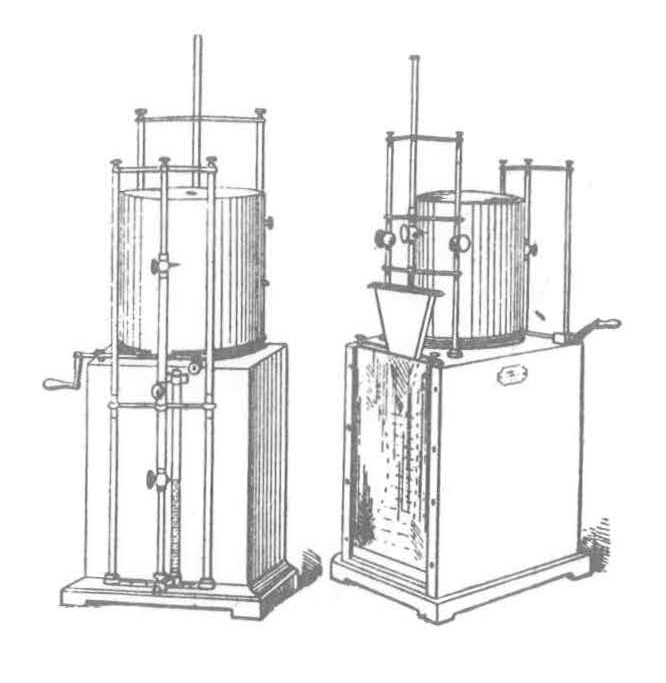
\includegraphics[scale=1.5]{h1.jpg}
\end{center}
\caption{Petrovićeva skica hidrointegratora. }
\label{fig:h1}
\end{figure}

\bigskip







\section{Primeri analognih računara}
\label{sec:naslov1}

U najpoznatije i najbitnije analogne računare spadaju:
	\begin{itemize}
		\item Logaritmar
		\item Al-Jazarijev sat u zamku
 		\item Diferencijalni analizator
		\item Analogni analizator
		\item Brzinomer
		\item Analogni sat
	\end{itemize}

\subsection{Logaritmar}
\label{subsec:podnaslov1}

Logaritmar je jedan od najosnovnijih analognih računara koji je kreiran u ranom 17. veku od strane Viliama Otreda (William Oughtred). U početku se koristio za množenje i deljenje, a nešto kasnije se pokazalo da je primenjliv za izračunavanja eksponencijalnih, logaritamskih i trigonometrijskih funkcija takođe.

Sastoji se od dve letvice istih dužina od kojih šira ima u sebi usečen žleb po kojem klizi uža letvica. Povrh šire letvice takođe po žlebu klizi providna pločica na kojoj je ucrtana tanka linija koja služi za isčitavanje rezultata. Na obe letvice je upisano više redova brojeva koji služe za računanje.
Računanje se sprovodi pomeranjem uže letvice duž šire, pri čemu se nad zadatim brojevima vrše razne operacije.
Navodno, prva posada koja je sletela na površinu meseca, predvođena Nil Armstrongom (Neil Armstrong), ponela je sa sobom razne elektronske sprave, uključujuci i logaritmar.

\subsection{Al-Jazarijev sat u zamku}
\label{subsec:podnaslov2}

Al-Jazarijev sat je starinski sat, visok skoro 3.5 metra, koji je koristio neke od složenih koncepata mašinstva za svoj rad. Osim prikazivanja vremena, bio je u mogućnosti da obavlja i druge funkcije kao što je prikazivanje solarnih i lunarnih orbita. Kreiran od strane Ismail al-Jazaria (Ismail al-Jazari), sat u zamku, jedan je od najvećih izuma svih vremena. Sagrađen je tokom prve decenije 13. veka. 

\subsection{Diferencijalni analizator}
\label{subsec:podnaslov3}

 Diferencijalni analizator su izmislila dva inženjera, Vanevar Buš (Vannevar Bush) i Harold Hejlzen (Harold Hazen), tokom ranih 1930-ih. Dizajniran je za rešavanje složenih diferencijalnih jednačina. Ova tehnologija koristi mehaničke aranžmane za obradu podataka i izračunavanje rešenja.

\subsection{Analogni termometar}
\label{subsec:podnaslov4}

Analogni termometar koristi stepenastu skalu i svojstva žive da bi ispunio svoj rad. Živa, koje je teČna na sobnoj temperaturi, pri zagrevanju se Širi. Time se omogućava potrošacu da dijagnostikuje bolesno stanje tela. Temperatura tela je analogni signal. Stoga je termometar koji meri telesnu temperaturu odličan primer analognih računara. 

\subsection{Brzinomer}
\label{subsec:podnaslov5}

Brzinomer je uređaj koji detektuje brzinu vozila u pokretu, uglavnom u kilometrima po času. Brzina se pokazuje pomoću igle kojoj je dozvoljeno da se slobodno kreće u skladu sa analognim signalom koji prima. Kabl brzinomera je na jednom kraju pričvršćen za osovinu zupčanika, a na drugom kraju za trajni magnet. Ovaj magnet je povezan sa metalnom čašom za brzinu bez fizičke veze između njih. čaša za brzinu je povezana indikatorom pomoću induktorske šipke na kojoj je pričvršćena opruga. Vrteća spoljna osovina menjača rotira magnet. Magnetno polje koje generiše pokretni magnet privlači metalnu čašu brzine. Ovo mehaničko kretanje čašice za brzinu se koristi za skretanje igle. Ovaj otklon igle ukazuje na brzinu vozila.


\subsection{Analogni sat}
\label{subsec:podnaslov6}


Iako su digitalni satovi sve češće u upotrebi, tradicionalni, analogni satovi idalje obavljaju posao u mnogim domaćinstvima. Mnogi nisu ni svesni da je analogni sat oblik analognog računara. On koristi kristal kvarca koji je podložan piezoelektričnom efektu. Napon koji obezbeđuje baterija, analogni signal, omogućava piezoelektričnom kristalu da vibrira brzinom od tačno 32 768 vibracija u sekundi. Uz pomoć ovih vibracija, generiče se impuls, a jedan impuls je vremenski ekvivalentan jednoj sekundi. Dakle, jedna sekunda je jednaka 32 768 vibracija piezoelektričnog kristala.


\section{Istorijat}
\label{sec:naslovN}

Prvi najraniji primer analognog računara jeste mehanizam sa Antikitere napravljen u Grčkoj i koristila se za računanje pozicija astronomskih tela. Naziv Antikitera dobila je po tome što su naučnici nasli taj mehanizam na Grčkom ostrvu Antikitera i smatra se da je napravljen izmedju 150-100 godine pre nove ere. Zbog njegovog kompleksnog nacina upotrebe, ljudi su tragali za "mašinama" koje će da rade isti posao samo jednostavnije. 

\subsection{Nakon mehanizma sa Antiketire \ref{fig:h2}}
\label{subsec:podnaslovK}

U drugom veku nove ere konstruisana je masina pod nazivom astrolab i nedugo posle biće konstruisana još jedna mašina slična astrolabu koji nosi naziv planisfera. Astrolab i planisfera su imali slične primene, a to je da rešavaju većinu astroloških problema. Kasnije ce jedan iranski akademik da napravi astrolab koji će da radi preko zupčanika. Prvi programibilni analogni računar je napravljen u 13. veku pod nazivom astronomski časovnik. Nakon ovog otkrića, pojavljajuće se novi programibilni instrumenti koji ce da vrše neke druge funkcije, nekih od njih su sektor, planimetar, logaritmar, kalendar, predvitelj talasa i diferencijski analizator.

\begin{figure}[h!]
\begin{center}
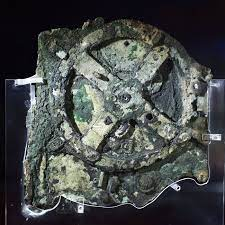
\includegraphics[scale=1]{MehanizamSaAntiketere.jpg}
\end{center}
\caption{Mehanizam sa Antikitere. }
\label{fig:h2}
\end{figure}

\pagebreak

\subsection{Moderno doba}
\label{subsec:podnaslovM}

Početkom 20. veka napravljen je dumaresk, sprava koja se koristila u mornarici. Par godina kasnije biće napravljena sprava slična dumaresku, stim što je ova sprava radila na struju. Ovu spravu je koristila Nemačka vojska u Prvom svetskom ratu. U periodu izmedju dva svetska rata imamo uredjaj napravljen 1929. godine nazvan mrežni analizator i on je funkcionisao koristeći naizmeničnu struju. Njena uloga je bila da rešava računske probleme vezane za električni sistem gde do tada nije moglo da se računa drugim metodama. U Drugom svetskom ratu imamo uredjaje (analogne računare) koje su se koristili ili kao oružje ili kao uredjaji za otkrivanje strateških značajnih pozicija. Nakon Drugog svetskog rata, analogni računari su se generalno pravili ili za prognoziranje nečega ili za izračunavanje komplikovanih matematičkih problema. U 2000-tim, analogni računari prelaze sa mehaničkih integratora i vakuumskih cevi na mikroprocesore.

\section{Podela prema nameni}
\label{sec:naslovcic}

Analogni računari se mogu podeliti prema nameni na:
	\begin{itemize}
		\item Specijalne
		\item Univerzalne
		\item Kombinovane
	\end{itemize}

\subsection{Specijalne}
\label{subsec:podnaslovS}

Koriste se za rešavanje problema tipa prenosa toplote, protoka tečnosti, opterećenja struje... Termalni analizator je jedan od primera analognog računara sa ovakvim tipom namene i imala bi otpornike, kondenzatore i posebne jedinice za proračun. Drugačiji naziv za ovaj tip je i pasivni analogni računari.

\subsection{Univerzalne}
\label{subsec:podnaslovU}

Njihov zadatak je bio da rešavaju sisteme diferencijalnih jednačina, uključujući sisteme linearnih ili nelinearnih jednačina sa više promenljivih. Za rešavanje linearnih koristili su se množači, sabirači, delitelji, integratori i merni sistemi, dok za nelinearne se koristili generatori funkcija.

\subsection{Kombinovane}
\label{subsec:podnaslovK}

Kombinovani direktne i indirektni analogni računari se koriste za simulacije u realnom vremenu.

\section{Podela analognih računara prema načinu dobijanja rešenja}
\label{sec:naslovcina}

Analogni računari se mogu podeliti prema načinu dobijanja rešenja na:

	\begin{itemize}
		\item Spori
		\item Repetitivni
	\end{itemize}

\subsection{Spori}
\label{subsec:podnaslovspori}

Promenljiva t se može birati po želji, pa čak i u realnom vremenu. Prednost sporih analognih računara je to što se izvršava u realnom vremenu, dok im je mana to što se početni uslovi mogu menjati samo na početku 

\subsection{Repetitivni}
\label{subsec:podnaslovrepetivni}

Rade na frekvenciji 50-60 Hz i ponavljaju rešenje toliko puta u sekundi. Svaka promena parametra se odražava na rezultat i zbog toga je potrebna provera i praćenje rada.

\newpage

\section{Elektronski analogni računari}
		\label{sec:naslov8}
		
		\bigskip
		
		\par Mane mehaničkih analognih računara kao što su:
		\begin{itemize}
			\item njihova veličina i veoma zahtevno održavanje
			\item brzina izračunavanja ograničena momentom inercije komponenata
			\item limitirana preciznost na svega nekoliko procenata usled mrtvog hoda
			\item dug vremenski interval potreban za podešavanje računara za specifične probleme jer je blio potrebno izvršiti veliki broj prespajanja
		\end{itemize}
		bile su samo neki od razlog za kratak životni vek mehaničkih analognih računara i rađanja ideje o \emph{elektronskim analognim računarima} koji su brzo postali veoma uticajani.
		
		\bigskip
		
		\par Prvi elektronski analogni rčunar implementirao je nemački naučnik Helmut Helcer (nem. Helmut Hölzer) sredinom Drugog svetskog rata tokom svog rada na kontroli letenja namenskog dalekometnog artiljerijskog oružja za strateško bombardovanje što je zahtevalo ogroman broj izračunavanja. \cite{Holzer}
		
		\bigskip
		
		\par Ključna stavka ovakvih računara je \emph{operacioni pojačavač}: komponenta u elektronskom kolu, sa dva ulazna i jednim izlaznim signalom, koja ima za cilj da pojača izlazni signal povećanjem razlike potencijala između dva ulazna signala. Prvobitno, ovaj uređaj bio je dizajniran za potrebe američke transkontinentalne telefonije. Druga bitna komponenta ovih računara bio je potenciometar koeficijenta korišćen da obezbeti odgovarajuće skaliranje elektronskih analognih promenljivih.
		
		\bigskip
		
		\par Rani elektronskii analogni računari brzo su stekli popularnost, a razlozi tome bili su:
		\begin{itemize}
			\item manja veličina u odnosu na mehaničke analogne računare (slika \ref{fig:aVSe})
			\item lakša prenosivost
			\item niža cena
			\item  veća brzina
		\end{itemize}
		Još jedan od razloga njihove popularnosti je taj što su ubrzo postali nerazdvojni deo istraživanja i razvijanja projekata u vojsci, vazduhoplovstvu i centrima za inženjerska istraživanja, što pokazuje i tabela \ref{tab:tableEAR} \cite{table}
		
		\bigskip
		
		\begin{figure}[!h]
				\begin{minipage}[h]{2 in}
					\centering
					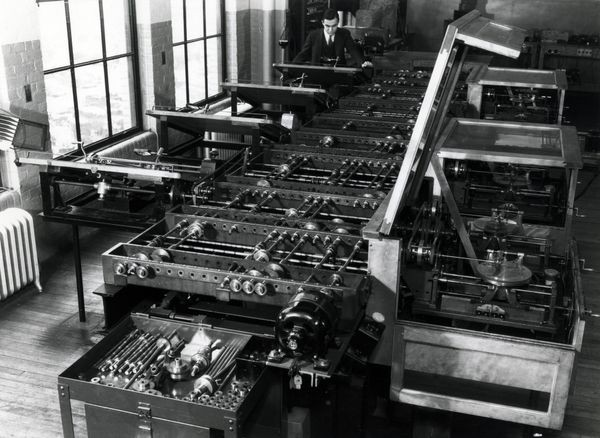
\includegraphics[scale = 0.2]{mehanicki.jpg}
				\end{minipage}
				\hfill
				\begin{minipage}[h]{2in}
					\centering
					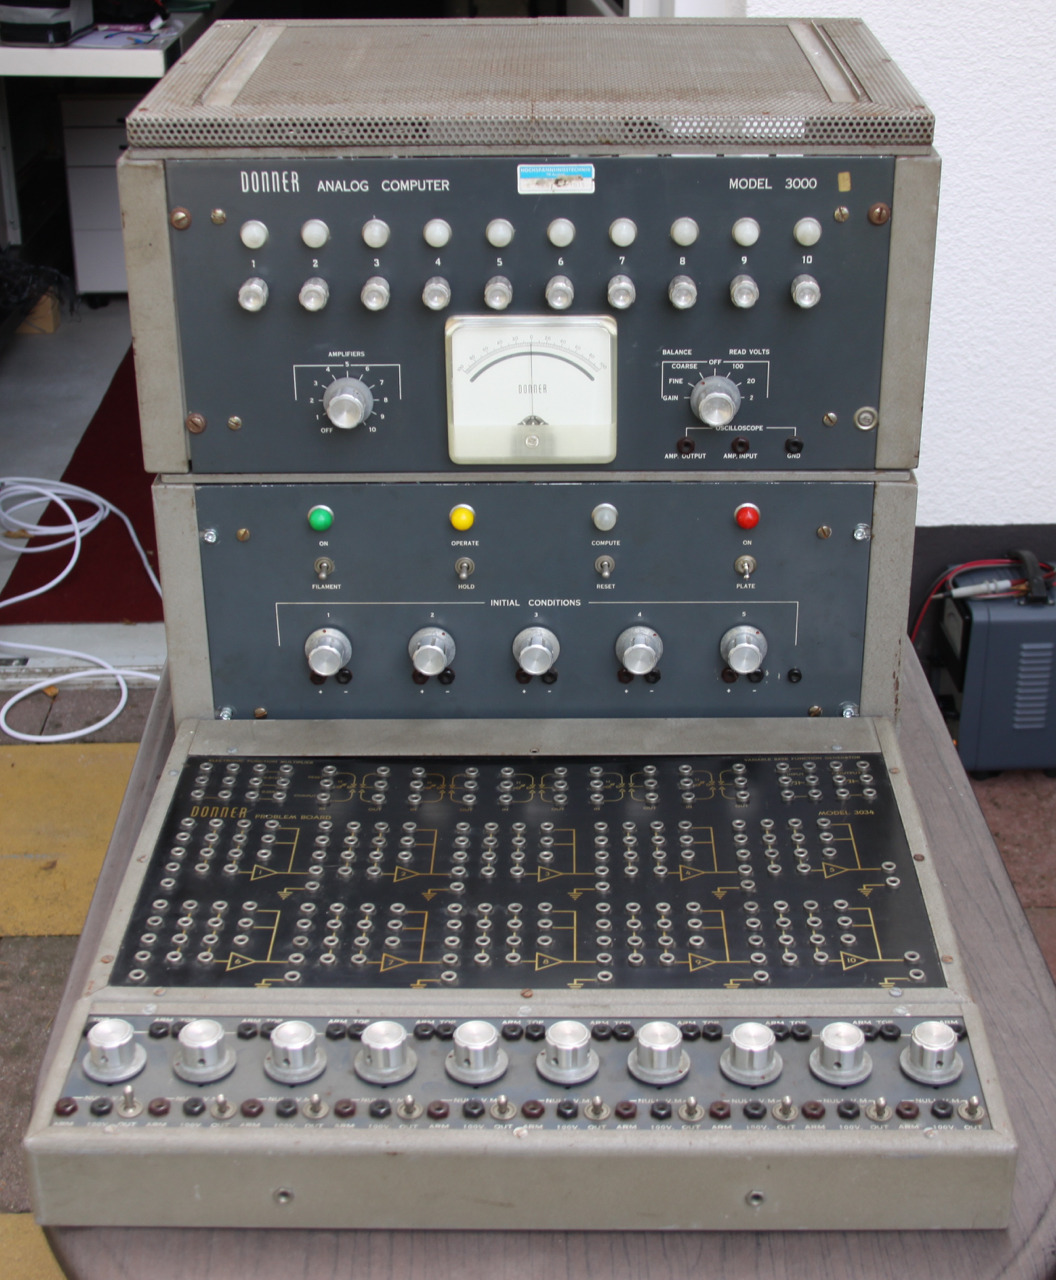
\includegraphics[scale = 0.067]{elektronski.jpg}
				\end{minipage}

				\caption{Odnos u veličini između mehaničkih (slika levo) i elektronskih (slika desno) analognih  računara.}
				\label{fig:aVSe}
		\end{figure}

		\begin{table}[h!]
			\begin{center}
				\begin{tabular}{| m{2cm} | m{4cm} | m{1cm} | m{4cm} |}
					\hline
					Projekat /mašina & Razvojni centar & Datum & Namena \\
					\hline
					Projekat \emph Ciklon & Američka mornarica & 1946 & analogno - digitalno praćenje performansi \\
					\hline
					Projekat \emph Tajfun & Američka mornarica / RCA & 1947 & Jednostruka namenska mašina \\
					\hline
					MIT simulator letenja & Američka mornarica/MIT & 1948- 1958 & \\
					\hline
					RAND analogni računar & RAND korporacija & 1948 & Pravljenje Rand analognog računara \\
					\hline
					GEDA/BEAC &  Američka avijacija & 1950 & program balističkih projektila \\
					\hline
					TRIDAC & RAE/ Elliot Brothers ltd. & 1950- 1955 & Simulacija lansiranja projektila \\
					\hline
					LACE & Engleska elektroindustrija & 1953- 1956 & Opšta namena/simulacija lansiranja projektila \\ 
					\hline
				\end{tabular}
				\label{tab:tableEAR}
				\caption{
						Akronimi iz tabele: \\
						\textbf{RCA} (\textit eng. \textbf Radio \textbf Corporation of \textbf America) - Američka radijska korporacija \\
						\textbf{MIT} (\textit eng. \textbf Massachusetts \textbf Institute of \textbf Technology) - Tehnološki institut u Masačusetsu  \\
						\textbf{RAND} (\textit eng. \textbf Research \textbf{an}d \textbf development) - Američki istraživački centar za globalnu politiku \\
						\textbf{GEDA} (\textit eng. \textbf Goodyear \textbf Electronic \textbf Differential \textbf Analyzer) - Elektronski diferencijalni analizator aviokompanije Gudjir \\
						\textbf{BEAC} (\textit eng. \textbf Boeing \textbf Electronic \textbf Analog \textbf Computer) - Elektronski analogni računar kompanije Boing \\
						\textbf{TRIDAC} (\textit eng. \textbf {Three}-\textbf Dimensional \textbf Analogue \textbf Computer) - Britanski elektronski analogni računar korišćen u vojnom vazduhoplovstvu \\
						\textbf{LACE} (\textit eng. \textbf Luton \textbf Analogue \textbf Computing \textbf Engine) - Britanski vojni analogni računar opšte namene proizveden u odseku za elektronsko navođenje projektila u Lutonu 
						}
			\end{center}
		\end{table}

		\pagebreak
		
		

\addcontentsline{toc}{section}{Literatura}
\appendix

\iffalse
\bibliography{seminarski} 
\bibliographystyle{plain}
\fi



\begin{thebibliography}{9}



\bibitem{antikitera} Jo Marchant, "Archimedes and the 2000-year-old computer" New Scientist, 12 December 2008.

\bibitem{tide} E G Fischer (1912), "The Coast and Geodetic Survey Tide Predicting Machine No. 2".

\bibitem{hidrointegrator} Srpska akademija nauka i umetnosti, "Hidrointegrator Mihaila Petrovića Alasa". Pristupljeno 6.11.2022.

\bibitem{Holzer} Thomas H. Lange. \emph{Peenemuende, Analyse einer Technologieentwicklung im Dritten Reich}. VDI-Verlag, Dusseldorf, 2006.
			
\bibitem{table} Bissell, C.C. (2004). \emph{A great disappearing act: the electronic analogue computer}. IEEE Conference on the History of Electronics, Bletchley, UK, 28-30 Jun 2004.


\end{thebibliography}


\end{document}
